% -*- root: ../EstadisticaII.tex -*-
\chapter{Clasificación}


Disponemos de una muestra de $k$ variables medidas en $n$ unidades u objetos que pertenecen a dos grupos o poblaciones \textit{(training data)}.

Cada observación $i=1,\ldots,n$ consiste en un vector $(x'_i,y_i)'$, donde $x_i\in\mathbb{R}^k$ son las $k$ variables e    $y\in\{0,1\}$ indica el grupo al que pertenece la unidad en la que se han obtenido. 

\textbf{Objetivo:} Asignar una nueva unidad con valores $x$ (e $y$ desconocida) a uno de los dos grupos (\textbf{obtener una regla de clasificación}).


Este problema tiene diferentes nombres en la literatura en inglés: ``supervised classification", ``statistical learning", ``discrimination", ``machine learning", ``pattern recognition", etc.

Vamos a ver un ejemplo, para entender mejor el tema

\begin{example}
En un estudio de factores de riesgo en enfermedades coronarias, se dispone de datos de 462 personas (de las que 160 habían sufrido infartos y 302 eran controles). Para cada una de ellas se midieron las siguientes variables:


\begin{center}
\label{example:infartos}
{\scriptsize

\begin{tabular}{|c|l|}
\hline Nombre variable & Descripci\'{o}n  \\
\hline {\tt sbp} & Tensión sanguínea sistólica \\
{\tt tobacco} & Consumo de tabaco\\
{\tt ldl} & Colesterol\\
{\tt adiposity} & Medida de adiposidad\\
{\tt typea} & Comportamiento ``tipo A"\\
{\tt obesity} & Medida de la obesidad\\
{\tt alcohol} & Consumo de alcohol\\
{\tt age} & Edad \\
 \hline
 \end{tabular}

 }
\end{center}

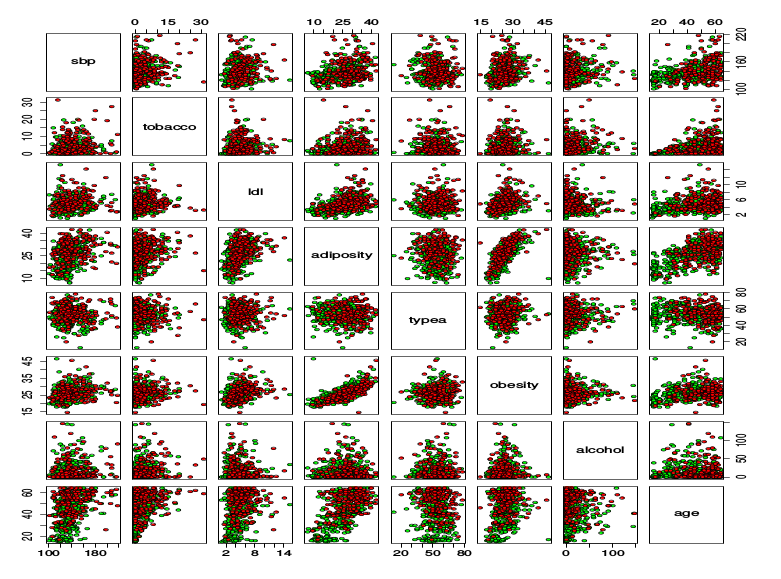
\includegraphics[width=13 cm]{img/pairs-heart.png}


Ahora nos gustaría poder predecir si un nuevo individuo va a tener un infarto o no en función de su consumo de tabaco, colesterol, ...
\end{example}


\section{Regla de Mahalanobis}

La idea es asignar el nuevo individuo al grupo cuyo centro es más cercano (cercano en el sentido de la distancia de Mahalanobis).


\begin{defn}[Regla\IS de Mahalanobis]
Para $i=0,1$ denotamos $P_i$  a la distribución condicionada  $X|Y=i$. Suponemos que $P_i$ es una distribución con vector de medias $\mu_i$ y matriz de covarianzas $\Sigma_i$.


\textbf{Regla de Mahalanobis:} Clasificar $x$ en el grupo 1 (i.e. $Y=1$) si y solo si
\[
(x-\mu_0)'\Sigma_0^{-1}(x-\mu_0) >  (x-\mu_1)'\Sigma_1^{-1}(x-\mu_1).
\]
\end{defn}
En la práctica se usan los vectores de medias y las matrices de covarianzas muestrales, ya que no disponemos de los reales.

La frontera de clasificación sería cuando 
\[
(x-\mu_0)'\Sigma_0^{-1}(x-\mu_0) =  (x-\mu_1)'\Sigma_1^{-1}(x-\mu_1).
\]

Esta frontera será una curva cuadrática (por ser una igualdad entre formas cuadráticas). 

\begin{example}


\centerline{$\mu_0=(1,0)^\prime$, $\mu_1=
(5,0)^\prime$, $\Sigma_1=\left[
  \begin{array}{cc}
    1 & 0 \\
    0 & 1 \
  \end{array} \right]$,
$\Sigma_2=\left[
  \begin{array}{cc}
    5 & 0 \\
    0 & 5 \
  \end{array} \right]$.}

\begin{center}
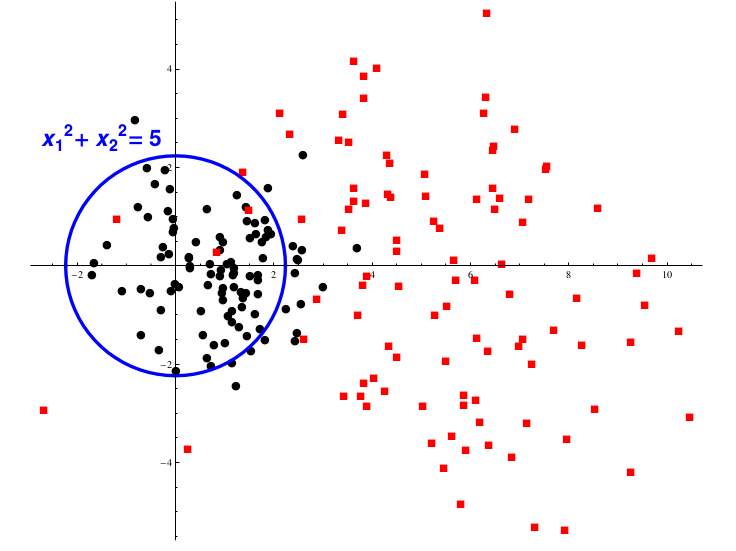
\includegraphics[width=13 cm]{img/ReglaMahalanobis.png}
\end{center}

\end{example}

\section{Regla de Fisher}

Vamos a suponer $Σ_1 = Σ_0$, que es cuando mejor funciona esta regla. Vamos a suponer que tenemos estos datos:

\begin{center}
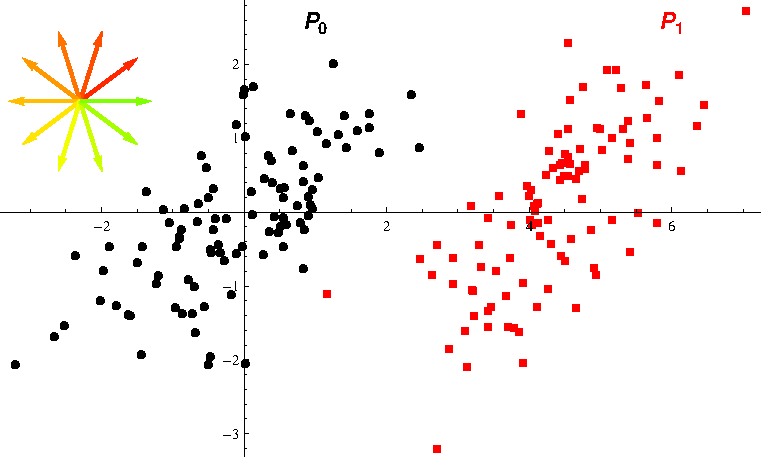
\includegraphics[width=13 cm]{pdf/tema4/_Fisher}
\end{center}


Y la idea intuitiva es construir una recta sobre la que proyectar, para construir 2 histogramas. Si nos dan un nuevo dato, lo clasificaremos en el histograma al que sea más probable que pertenezca.

\begin{center}
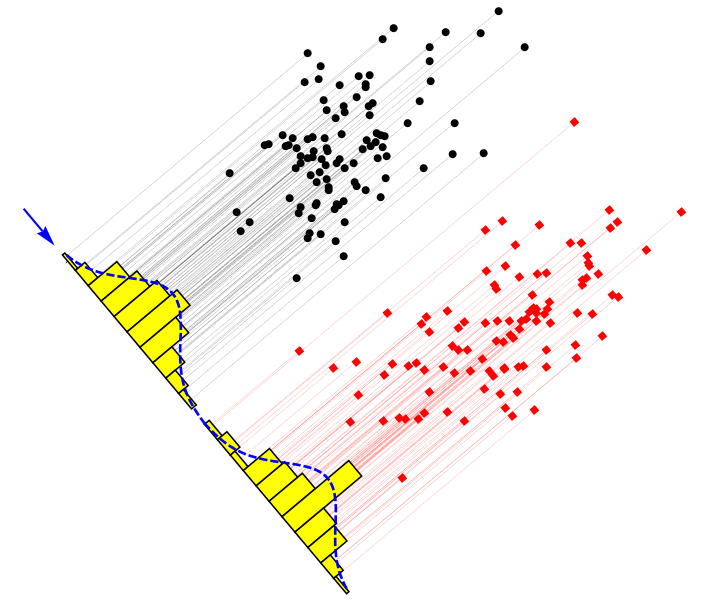
\includegraphics[width=13 cm]{img/ReglaFisherIntuitiva.png}
\end{center}


\paragraph{¿Cómo construir esta recta?} Tenemos que tener en cuenta 2 cosas:


\begin{itemize}
  \item Una buena direcci\'{o}n debe separar bien los centros de los grupos. La distancia entre las medias $(a'\mu_0-a'\mu_1)^2 = a'Ba$, donde $B=(\mu_0-\mu_1)(\mu_0-\mu_1)'$, debe ser grande.

\centerline{{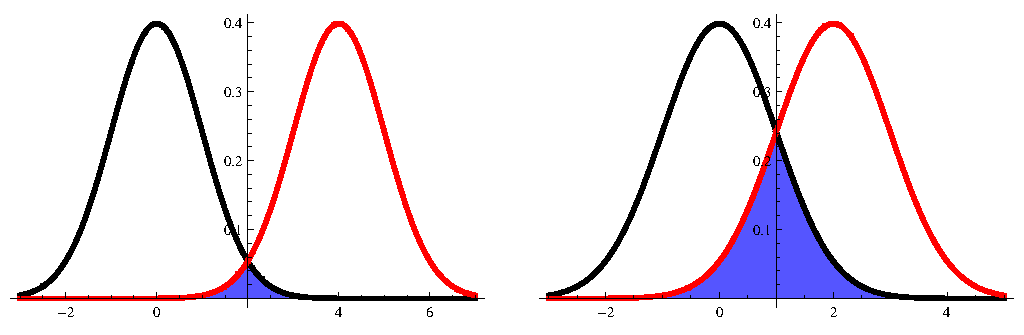
\includegraphics[width=13 cm]{pdf/tema4/_Fisher-normales-1}}}

  \item La varianza de las proyecciones dentro de los grupos ($a'\Sigma a$) debe ser lo menor
  posible.

\centerline{{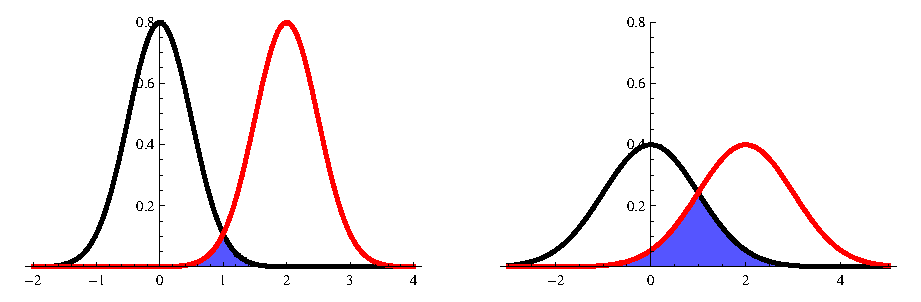
\includegraphics[width=13 cm]{pdf/tema4/_Fisher-normales-2}}}

\end{itemize}


La idea de Fisher fue maximizar el ratio de la separación de los centros entre las varianzas, es decir, maximizar el \concept{Cociente\IS de Rayleigh}

\[
f(a) = \frac{a'Ba}{a'\Sigma a} 
\]

para cualquier dirección $a∈ℝ^n$.

\obs Este problema tiene infinitas soluciones, ya que $f(a) = f(λa) ∀λ∈ℝ$. Para solucionar esto, imponemos la normalización tal que $a'Σa = 1$ (aunque no sea la única).

Vamos a calcular el máximo de esta función\footnote{Utilizamos $\grad a'Σa = 2aΣ$. La derivada de una forma cuadrática que es algo que ya deberíamos haber sabido de otras asignaturas del grado.}

\[
\grad f(a) = \frac{2Ba(a'Σa) - 2Σa(a'Ba)}{(a'Σa)^2} \to \grad f(ω) = 0 \dimplies Bω(ω'Σω) = Σω(ω'Bω)
\]

Si llegamos a encontrar ese $ω$, tendrá estas 2 propiedades
\begin{itemize}
	\item $Bω = (µ_0-µ_1)\underbrace{(µ_0 - µ_1)'ω}_{α}$ siendo $α$ un escalar. Esto quiere decir que $Bω = (µ_0-µ_1)α$, esto es: $Bω$ es proporcional a $µ_0 - µ_1$. 
	\item $Σω$ es proporcional a $Σ^{-1}(µ_0 - µ_1)$
\end{itemize}

\begin{defn}[Regla\IS de Fisher] Clasificar $x$ en el grupo 1 (i.e. $Y=1$) si y solo si
\[
ω'\left(x-\frac{\mu_0 + \mu_1}{2}\right)>0
\]
donde $ω=\Sigma^{-1}(\mu_1-\mu_0).$

En caso de tener $ω'\left(x-\frac{\mu_0 + \mu_1}{2}\right)<0$, clasificaríamos en el grupo 2.
\end{defn}

\obs Si en la regla de Mahalanobis se supone $Σ_1 = Σ_2$, se obtiene la regla de Fisher:
\begin{align*}
  ω'\left(x-\frac{\mu_0 + \mu_1}{2}\right) &> 0\\
  (μ_1 - μ_0)' Σ^{-1} \left( x - \frac{\mu_0 + \mu_1}{2} \right) &> 0\\
  (μ_1 - μ_0)' Σ^{-1} x - (μ_1 - μ_0)' Σ^{-1} \left(\frac{\mu_0 + \mu_1}{2} \right) &> 0\\
  (μ_1 - μ_0)' Σ^{-1} x - \underbrace{μ_1'Σ^{-1}\frac{μ_0}{2}}_{A} + μ_0'Σ^{-1}\frac{μ_0}{2} - μ_1'Σ^{-1}\frac{μ_1}{2} + \underbrace{μ_0'Σ^{-1}\frac{μ_1}{2}}_{B} &>0
\end{align*}
Sabiendo $A,B∈ℝ \implies A=A^T=B$ podemos seguir:
\begin{align*}
  2(μ_1 - μ_0)' Σ^{-1} x + μ_0'Σ^{-1}μ_0 - μ_1'Σ^{-1}μ_1 &>0\\
  x'Σ^{-1}(μ_1-μ_0) + (μ_1-μ_0)'Σ^{-1}x + μ_0'Σ^{-1}μ_0 - μ_1'Σ^{-1}μ_1 &>0\\
  x'Σ^{-1}x - x'Σ^{-1}μ_0 - μ_0'Σ^{-1}x + μ_0'Σ^{-1}μ_0 &> x'Σ^{-1}x - x'Σ^{-1}μ_1 - μ_1'Σ^{-1}x + μ_1'Σ^{-1}μ_1\\
  (x'Σ^{-1} - μ_0'Σ^{-1})(x - μ_0) &> (x'Σ^{-1} - μ_1'Σ^{-1})(x-μ_1)\\
  (x-μ_0)'Σ^{-1}(x-μ_0) &> (x-μ_1)'Σ^{-1}(x-μ_1)\\
\end{align*}
Por tanto hemos llegado a la regla de Mahalanobis desde la regla lineal de Fisher suponiendo que $Σ_1 = Σ_2$.

\obs Esta regla funciona bien cuando $Σ_0 = Σ_1$, es decir, las nubes de puntos tienen la misma forma y orientación. ¿Qué ocurre cuando las matrices de covarianzas son distintas?

\begin{center}
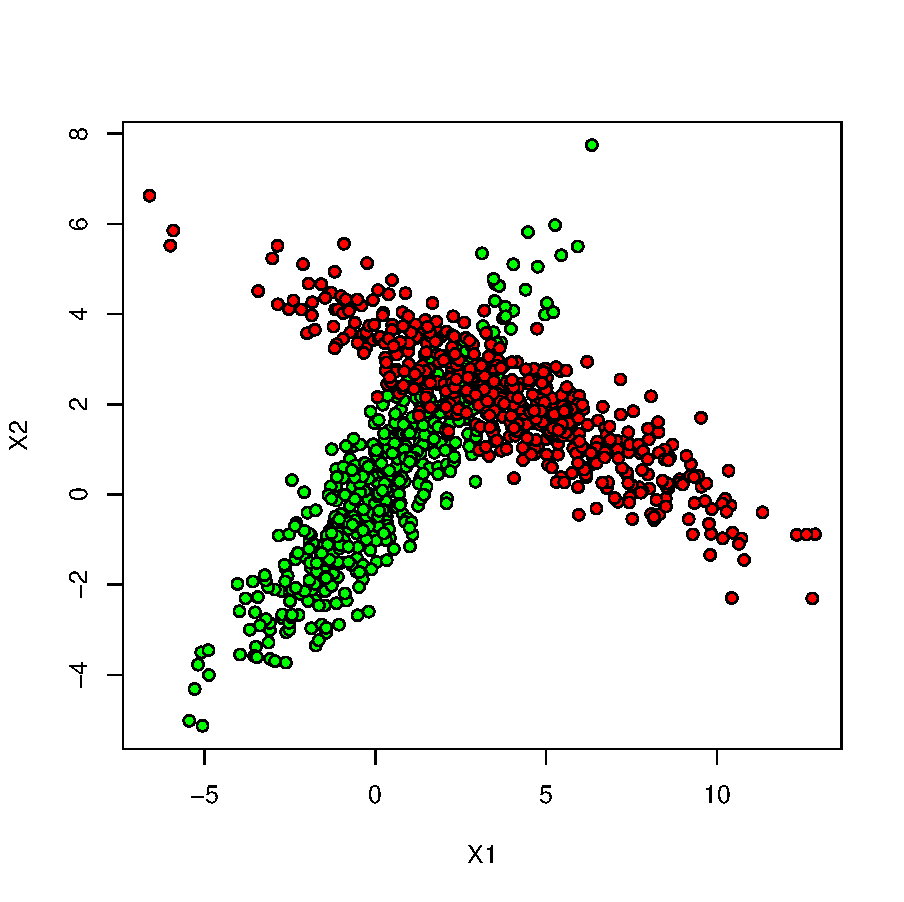
\includegraphics[width=13 cm]{pdf/tema4/_sim-plot}
\end{center}

En la imagen vemos que la regla de Fisher (recta azul) no divide nada bien los datos. Por otro lado, vemos la división por la distancia de Mahalanobis (en rojo) que es mucho más adecuada.

\begin{center}
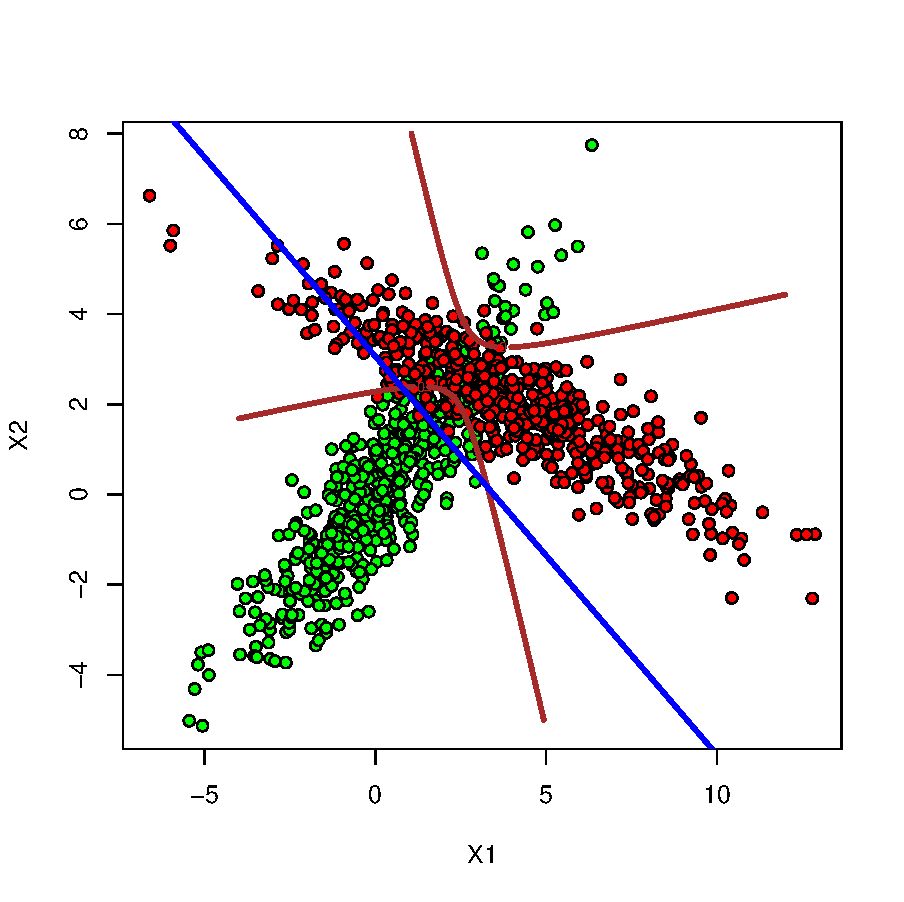
\includegraphics[width=13 cm]{pdf/tema4/_sim-plot-reglas}
\end{center}


\subsection{Validación del modelo}

Acabamos de ver un ejemplo de un caso en el que vemos (a simple vista) que un modelo clasifica mejor que el otro. ¿Porqué sabemos que es mejor? Porque comete menos errores. Vamos a ver en esta sección cómo calcular errores.

\centerline{{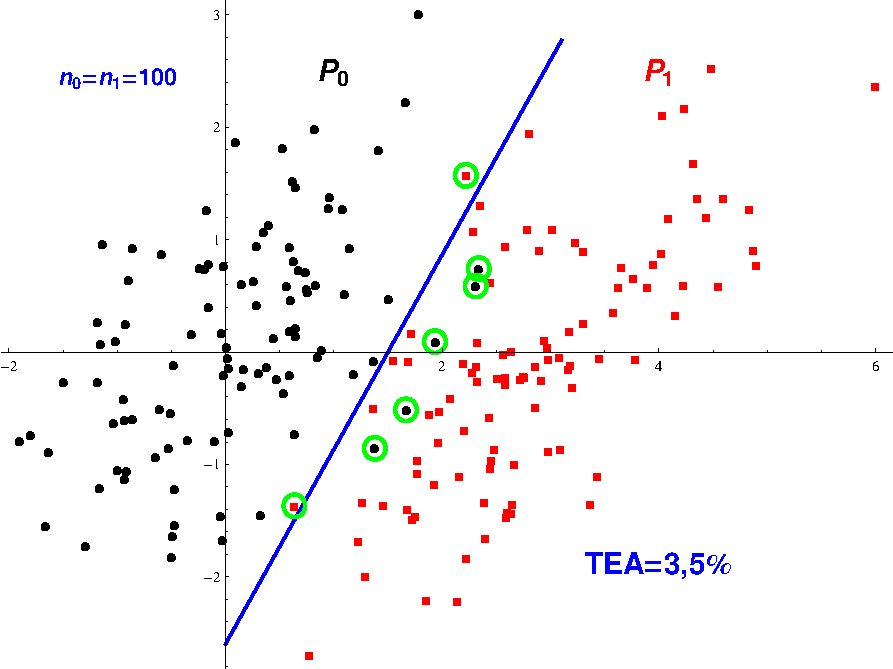
\includegraphics[width=13 cm]{pdf/tema4/_errores-1}}}

\begin{defn}[Tasa de error aparente]
$$\text{TEA}:=\frac{\text{Total de mal clasificados en la muestra}}{n}100\%.$$
\end{defn}

El problema de esta tasa de error es que infraestima la tasa de error. Esto se debe a que estamos utilizando los mismos puntos para construir el modelo y para evaluarlo. 

La solución es la creación de particiones de train y de test. De esta manera utilizamos los datos de train para construir el modelo y el de test para evaluarlo. ¿Y cómo asegurar que la tasa de error no depende de las particiones construidas? No se puede, pero lo que podemos hacer es utilizar la Validación cruzada.

\begin{defn}[Validación\IS cruzada]Omitimos un dato de los n observados y generamos la regla de clasificación con los n − 1 restantes. Clasificamos la observación apartada y repetimos el procedimiento para cada una de las observaciones.
\end{defn}


\section{Regresión logística}

Vamos a recordar el ejemplo de infartos de miocardio y vamos a ver cómo clasifican los modelos de clasificación estudiados hasta ahora.

En rojo vemos utilizando la distancia de Mahalanobis y en azul la regla de Fisher.
\centerline{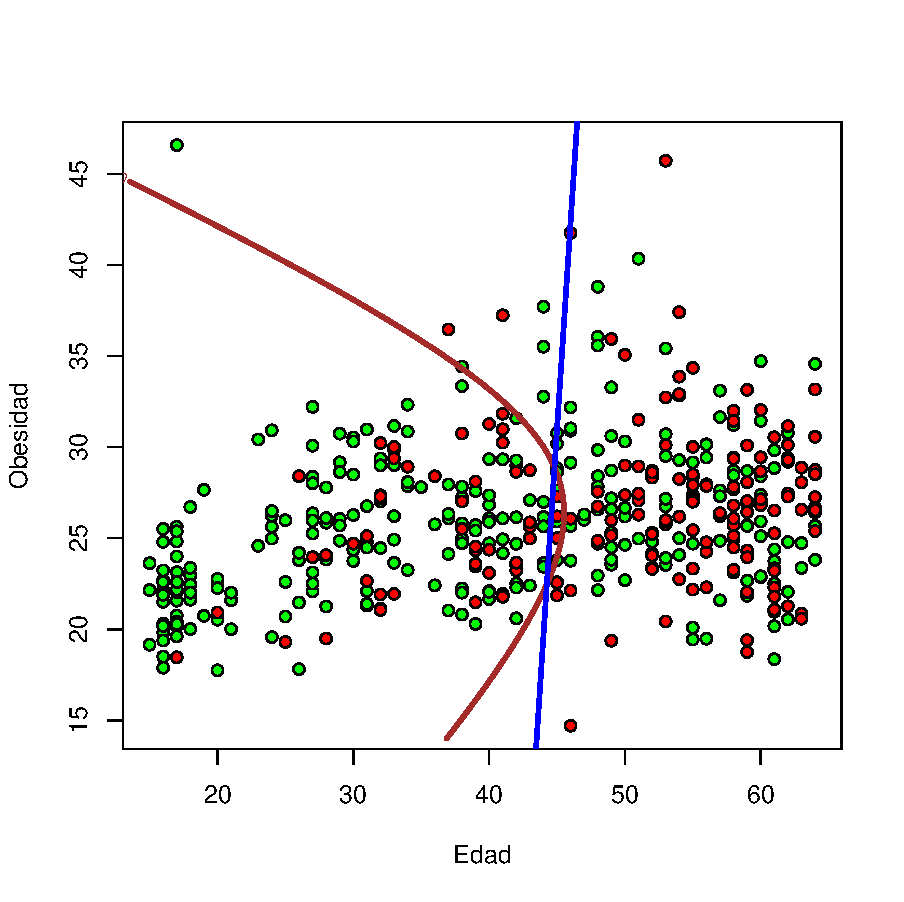
\includegraphics[width=13 cm]{pdf/tema4/_edadobesidad-reglas}}

Vemos que ninguno de los 2 es bueno. Por ello, vamos a ver otro método de clasificación planteando  la clasificación como un problema de regresión múltiple. 

No podemos utilizarlo como tal porque la variable regresora $Y_i$ es binaria y en la regresión múltiple era continua (más concretamente normal). Por ello, hay que buscar una alternativa.


\subsection{Construcción del modelo}
Las variables $Y_1,\ldots,Y_n$ son independientes y tienen distribución de Bernoulli. 

Denotamos $p_i=\mathbb{P}(Y_i=1 \mid x_i)$. La probabilidad de ``éxito'' depende de las variables regresoras.

Una relación lineal $p_i=\beta_0+\beta_1x_{i1}+\cdots+\beta_kx_{ik}$ no es adecuada\\ (¿por qué?)

Suponemos que la relación entre $p_i$ y $x_i$ viene dada por 
\[p_i = \frac{1}{1+e^{-\beta_0-\beta_1x_{i1}-\cdots-\beta_kx_{ik}}},\]
es decir,
\[p_i = F(\beta_0+\beta_1x_{i1}+\cdots+\beta_kx_{ik}),\]

donde $F(x)=1/(1+e^{-x})$ es la \concept{Función\IS logística}.


\obs 

\begin{itemize}
  \item \[F(-x) = \frac{1}{1+e^{x}} = \frac{e^{-x}}{1 + e^{-x}} = 1 - F(x)\]
  \item \[F'(x) = \frac{e^{-x}}{(1+e^{-x})^2} = F(x)(1-F(x))\]
  \item \[\log\frac{p_i}{1-p_i} = β'x_i\]
\end{itemize}


\begin{defn}[Razón\IS de probabilidades]
Llamamos $O_i$ a la \textbf{razón de probabilidades} para la observación $i$:
\[
 O_i=\frac{p_i}{1-p_i} 
\]
\end{defn}
\paragraph{Interpretación} El estado de las apuestas. 


\paragraph{¿Cómo varía la razón de probabilidades si la variable regresora $x_{ij}$ se incrementa una unidad?}

Si se cumple el modelo de regresión logística, entonces
\[
O_i =  e^{\beta_0  + \beta_1x_{i1} + \cdots + \beta_kx_{ik}}
\]

Con lo que la variación:

\[
\frac{O'_i}{O_i} = \frac{e^{\beta_0+\cdots+\beta_j(x+1)+\cdots+\beta_kx_{ik}}}{e^{\beta_0+\cdots+\beta_jx+\cdots+\beta_kx_{ik}}}= e^{\beta_j}.
\]  
Por tanto $e^{\beta_j}$ es la variación de la razón de probabilidades cuando la variable regresora $j$ se incrementa en una unidad y el resto de variables permanece constante. 


\subsection{Estimación de los parámetros}


Para estimar los parámetros se usa el método de máxima verosimilitud.



Por ejemplo, si observamos los datos

\begin{center}
\begin{tabular}{c|ccc}
$x_i$ & 2 & 1 & 3 \\  \hline
$Y_i$ & 0 & 1 & 1
\end{tabular}
\end{center}

entonces $\hat{\beta}_0$ y $\hat{\beta}_1$ son los valores que maximizan la función de verosimilitud

%TODO: una pequeña explicación.

\[
L(\beta_0,\beta_1) = P(Y=0 \mid x = 2)P(Y=1 \mid x = 1)P(Y=1 \mid x = 3)
\]
\[
L(\beta_0,\beta_1) = \left(1-\frac{1}{1+e^{-\beta_0-2\beta_1}}\right)
\left(\frac{1}{1+e^{-\beta_0-\beta_1}}\right)
\left(\frac{1}{1+e^{-\beta_0-3\beta_1}}\right)
\]

Se suelen aplicar métodos numéricos estándar de optimización ya que es difícil sacar los valores exactos.


La fórmula general es:

\[ L(β) = \prod_{i=1}^n p_i^{Y_i}(1-p_i)^{1-Y_i}\]

De esta manera, cuando $Y_i = 0$, entonces nos quedamos con el término $(1-p_i)$. Por otro lado, cuando $Y_i = 1$, tenemos el término $p_i$.


Vamos a derivar el logaritmos de la función de verosimilitud:

\[
l(β) = \log (L(β)) = \sum_{i=1}^n \left[ Y_i\log p_i + (1-Y_i)\log (1-p_i) \right]
\]

\[
\grad l(β) = \sum_{i=1}^n \left[ \frac{Y_i}{p_i} p_i(1-p_i)x_i - \frac{1-Y_i}{1-p_i}p_i(1-p_i)x_i \right] = \sum_{i=1}^n\left[  \right] = \sum_{i=1}^n (y_i-p_i)x_i
\]

En esta última cuenta podemos ver la conveniencia de la función logística. En realidad, podríamos utilizar cualquier otra función $F:ℝ \to [0,1]$. Utilizando otras funciones, no se tendrían estas simplificaciones que hacen relativamente fácil el cálculo del E.M.V. de $\vec{β}$


\paragraph{Conclusión:} $\hat{β}$ verifica:

\[
\sum(Y_i - \hat{p}_i)x_i = 0
\]
donde $p_i = \frac{1}{1 + e^{-\hat{β}'\vec{x}_i}}$

\subparagraph{Relación con regresión simple}

En regresión lineal simple, teníamos que el E.M.V. verifica: \[ \sum (Y_i - \hat{Y_i}) x_i = 0\] donde $\hat{Y_i} = \hat{β}'x_i$. 


\obs

\begin{enumerate}
  \item Recordamos que en el caso unidimensional, el E.M.V. tiene una distribución de media el valor verdadero y varianza $\frac{1}{I_F}$ donde $I_F$ es la información de Fisher y se calculaba derivando 2 veces la verosimilitud (más o menos)

  En el caso multidimensional, tenemos:

  \[
  \hat{B} \equiv N_{k+1}\left( β,(X'\hat{W}X)^{-1}\right)
  \]

  Teniendo \[\hat{W} = \begin{pmatrix}\hat{p_1}(1-\hat{p_1}) & 0 & \dots & \dots \\ 0 & \hat{p_2}(1-\hat{p_2}) & \dots & \dots \\ \vdots &\ddots & & \vdots \\ 0 & \dots & 0 & \hat{p_n}(1-\hat{p_n})
   \end{pmatrix}\]
  y siendo $X$ la matriz de diseño.
  \item Desviaciones:

    \[D_i^2 = -2\left[ Y_i\log \hat{p_i} + (1-Y_i)\log(1-\hat{p}_i)\right] \]

  $D_i$ mide la bondad de ajuste del modelo a la observación $i$. 

  \subitem $Y_i = 1 \to D_i^2 = -2\log \hat{p}_i$. De esta manera, si $\hat{p}_i \to 0$, entonces $D_i^2 \to ∞$, cosa que tiene toda la lógica del mundo. Si el modelo me da muy poca probabilidad de clasificarlo como enfermo, siendo enfermo entonces estoy muy desviado y el modelo se ajusta mal para esa observación. Si por el contrario, $\hat{p}_i \to 1 \implies D_i^2 \to 0$, es decir, si me da mucha probabilidad, entonces hay muy poca desviación.

  \item Todas las consideraciones anteriores sobre las desviaciones se podrían haber hecho sin multiplicarlo por el 2. Vamos a ver porqué aparece.

  Maximizar $l(β)$ es lo mismo que minimizar $-2·l(β)$. 

  \begin{defn}[Desviación\IS residual]
    Vemos que cada sumando de $l(β)$ el $D_i^2$ correspondiente multiplicado por $-2$, es decir:
    \[
      -2 l(β) = \sum D_i^2 = D^2
    \]
    Este sumatorio es la desviación residual
  \end{defn}
  \obs Igual que en regresión múltiple minimizábamos la suma de los residuos, en este, el E.M.V. minimiza la desviación residual. Análogamente, si el modelo tiene demasiadas variables esta desviación se reduce y provoca que demasiadas variables reduzcan este valor. Lo mismo ocurría con el coeficiente de determinación ajustado.

  La solución es construir una ``desviación residual ajustada'' que penalice los modelos complicados.

  \subitem Utilizamos el \concept{Criterio\IS de Información de Akaike (AIC)} 
\label{def:AIC}
    \[AIC = D^2 + 2(k+1)\]

    \begin{proof}
      Si alguien está interesado en saber cuál es la justificación teórica del sumando ``2(k+1)'', puede buscar el artículo de Akaike en el que se explica, porque es algo que ni el profesor sabe bien.
    \end{proof}
\end{enumerate}

\begin{example}

\begin{lstlisting}[style=mystyle]
# Numero de observaciones
n = 100

# Parametros
beta0 = 0
beta1 = 3

# Genera los datos
x = rnorm(n)
p = 1/(1+exp(-beta0-beta1*x))
y = rbinom(n,1,p)

# Ajusta el modelo
reg = glm(y~x,family=binomial)
summary(reg)

# # # # Y obtenemos: # # # #


Deviance Residuals:
    Min       1Q   Median       3Q      Max
-1.8340  -0.7598  -0.1568   0.7623   2.4224

Coefficients:
            Estimate Std. Error z value Pr(>|z|)
(Intercept)  -0.1157     0.2585  -0.447    0.655
x             2.7083     0.5854   4.627 3.71e-06 ***
---
Signif. codes:  0 '***' 0.001 '**' 0.01 '*' 0.05 '.' 0.1 ' ' 1

(Dispersion parameter for binomial family taken to be 1)

    Null deviance: 137.628  on 99  degrees of freedom
Residual deviance:  90.396  on 98  degrees of freedom
AIC: 94.396

Number of Fisher Scoring iterations: 5

\end{lstlisting}

\begin{itemize}
  \item Los errores típicos son los elementos de la diagonal de la matriz $X'\hat{W}X$.
  \item Ejemplos:
  \subitem $H_0 : β_0 = 0$

  Vemos el valor $-0.447$ y lo comparamos con la tabla de la normal, o en su defecto cogemos el p-valor $0.655$ y no rechazamos la hipótesis (cosa que está bien)

  \subitem  Para el $IC(β_1)$

  \[
    IC(β_1) = [2.70 \mp \underbrace{z_{α/2}}_{1.96}0.5859] = 
  \]

  ¿Y porqué utilizamos la $N$ y no una $t$ como siempre? 

  %TODO: contestar

  \item Como en este caso $k=1$, vemos que $AIC = 4 + (\text{Resudial deviance}) = 4+D^2$
  \item ¿Qué es la ``Null deviance''? 

    \begin{defn}[Null\IS deviance]
    Tomando $H_0 : β_1 = ... = β_k = 0$, la ``Null deviance'' es $D_0^2$ para este modelo reducido.
    \end{defn}

  \item \textit{Family = binomial} es el valor que utilizar para que sea regresión logística.

\end{itemize}

\end{example}

\subsection{Contraste de un modelo reducido}

Modelo completo ($M$) y un modelo reducido ($M_0$) que procede de imponer $p$ restricciones en el modelo completo y tenemos el contraste $H_0 : M_0$ es cierto.

Vamos a estudiar $D_0^2 - D^2$ (que siempre es negativo, ya que al aumentar el número de variables el máximo del E.M.V. es mayor)

\[
D_0^2 - D^2  = -2 \log L(\hat{β}^{(0)}) + 2 \log L(\hat{β}) = -2\log\frac{L(\hat{β}^{(0)})}{L(\hat{β})}\] 

Esto es un \concept{Cociente\IS de verosimilitudes}. 

Llamamos $\Lambda = \frac{L(\hat{β}^{(0)})}{L(\hat{β})}$ y además sabemos que $$-2\log\Lambda\xrightarrow[H_0]{d}\chi^2_p$$


¿Porqué sabemos que se distribuye como una $\chi^2$? Este es un resultado visto en \cite[IV.4.3]{ApuntesEstI}.

Entonces, la región de rechazo es: \[R = \{D^2_0 - D^2 > \chi^2_{p;α}\}\]


Vamos a verlo en el ejemplo de la salida de $R$.

$D_0 = 137.628$, con lo que $D_0^2 - D^2  = 47.2$ y $p = 99-98 = 1$, entonces:

\[
R = \{47.2 > \chi^2_{1;0.05}\}\to \text{ p-valor } \simeq 0
\]

\paragraph{Conclusión}

Para contrastar $H_0 : β_j = 0$ tenemos 2 posibilidades. La primera es el \concept{test\IS de Wald}\label{test:Wald} que es el que hace $R$ pero también podemos construir un \concept{test\IS de razón de verosimilitudes}\label{test:RV}, que es lo que acabamos de hacer. Como en el ejemplo de $R$ hay 2 coeficientes, $M_0$ es sólamente $β_1 = 0$.


\begin{example}

Para el siguiente resultado:

\begin{lstlisting}[style=mystyle]
reg1 = glm(Y ~ edad, family='binomial')
summary(reg1)


Call:
glm(formula = Y ~ edad, family = "binomial")

Deviance Residuals: 
    Min       1Q   Median       3Q      Max  
-1.4321  -0.9215  -0.5392   1.0952   2.2433  

Coefficients:
             Estimate Std. Error z value Pr(>|z|)    
(Intercept) -3.521710   0.416031  -8.465  < 2e-16 ***
edad         0.064108   0.008532   7.513 5.76e-14 ***
---
Signif. codes:  0 '***' 0.001 '**' 0.01 '*' 0.05 '.' 0.1  ' 1 

(Dispersion parameter for binomial family taken to be 1)

    Null deviance: 596.11  on 461  degrees of freedom
Residual deviance: 525.56  on 460  degrees of freedom
AIC: 529.56

Number of Fisher Scoring iterations: 4
\end{lstlisting}




Queremos calcular:
\begin{itemize}
  \item Modelo ajustado $P(\hat{y=1 | edad})$
  \item Interpretación.
  \item $H_0 : β_1 = 1$ con los 2 métodos conocidos, Wald y Razón de verosimilitudes (RV).
  \item IC para $e^{β_1}$
\end{itemize}

Vamos a verlo.

Recordamos que el modelo es:
\[P_i = P(Y_i =1 | X = x) = \frac{1}{1+e^{-β'x}}\] donde $Y_1,...,Y_n \sim B(1,p_i)$ independientes.

Entonces, \[P(\hat{y=1 | EDAD}) = \frac{1}{1+\exp(3.5217 - 0.0651 · EDAD)}\]

La \textbf{interpretación} tiene que ver con $e^{\hat{β_1}} = 1.066$. Si la edad se incrementa un año, ¿Cuánto aumentan las apuestas de tener un infarto? $\tilde{O_i} = 1.066·O_i$

Para el \textbf{contraste} con el método de \textbf{Wald}, rechazamos $H_0$ porque el p-valor del contrate $β_1 = 0$ es muy pequeño.

Para el \textbf{contraste} utilizando RV, tenemos: $D_0^2 - D^2 = 591.11 - 525.56 = 70.55$ y utilizamos el resultado que asintóticamente es una $\chi^2$, con lo que la región de rechazo:

\[R = \{D_0^2 - D^2 > \chi^2_{1;α}\}\]

Consultando las tablas, vemos que para casi cualquier $α$, rechazamos porque el p-valor (que no estamos calculando) debe de ser casi 0. 

Vamos a construir el \textbf{intervalo de confianza}.
\[IC_{0.95}(β_1) = [0.064 - 1.96 · 0.0085]\] 
Con lo que:
\[ IC_{0.95}(e^{β_1}) = [e^{0.064 - 1.96 · 0.0085},e^{-0.064 + 1.96 · 0.0085}] \] 

\end{example}


\obs Como hemos visto, tenemos 2 contrastes para una misma hipótesis. Son contrastes distintos que usualmente dan los mismo resultados. Se podrían ``cocinar'' un poco los datos para rechazar con un contraste y aceptar con el otro.


\subsection{Con 2 variables regresoras}

Ahora vamos a tomar el modelo con la edad y la obesidad. En este caso, el estadístico $D_0^2 - D^2 = 596.11 -525.55$ sirve para contrastar $H_0 : β_1 = β_2 = 0$ y se compara con $\chi^2_2$ (2 grados de libertad porque imponemos 2 restricciones).


Vamos a verlo:

\begin{lstlisting}[style=mystyle]

reg = glm(Y ~ edad+obesidad, family='binomial')
# # Recordamos:
# reg1 = glm(Y ~ edad, family='binomial')

summary(reg)

Deviance Residuals: 
    Min       1Q   Median       3Q      Max  
-1.4401  -0.9227  -0.5384   1.0905   2.2497  

Coefficients:
             Estimate Std. Error z value Pr(>|z|)    
(Intercept) -3.581465   0.742611  -4.823 1.42e-06 ***
edad         0.063958   0.008674   7.374 1.66e-13 ***
obesidad     0.002523   0.025934   0.097    0.923    
---
Signif. codes:  0 '***' 0.001 '**' 0.01 '*' 0.05 '.' 0.1  ' 1 

(Dispersion parameter for binomial family taken to be 1)

    Null deviance: 596.11  on 461  degrees of freedom
Residual deviance: 525.55  on 459  degrees of freedom
AIC: 531.55

Number of Fisher Scoring iterations: 4

\end{lstlisting}

Ahora comparamos si al añadir la obesidad obtenemos suficiente información. 

\begin{lstlisting}[style=mystyle]
anova(reg1, reg, test='Chisq')
Analysis of Deviance Table

Model 1: Y ~ edad
Model 2: Y ~ edad + obesidad
  Resid. Df Resid. Dev Df  Deviance P(>|Chi|)
1       460     525.56                       
2       459     525.55  1 0.0094552    0.9225
\end{lstlisting}

Al ser las desviaciones muy similares quiere decir que al añadir la obesidad no obtenemos suficiente información como para que merezca la pena añadirla. Es por ello que el p-valor es muy grande.

\section{Regresión logística como clasificador}

\begin{defn}[Regla de clasificación\IS logística]
Clasificar $x$ en el grupo 1 (i.e. $Y=1$) si y solo si
\[
\widehat{\mathbb{P}(Y=1|x)}>\widehat{\mathbb{P}(Y=0|x)}
\]
\end{defn}
Sustituyendo por la función logística tenemos una regla lineal (diferente en general a la de Fisher): Clasificar $x$ en el grupo 1 (i.e. $Y=1$) si y solo si
\[
\hat\beta_0 +\hat\beta_k x_1 + \ldots + \hat\beta_k x_k > 0.
\]

En el \textbf{ejemplo}, clasificamos a un individuo como enfermo si y solo si
\[
-3.58 + 0.064 \cdot \tt{edad} + 0.0025 \cdot \tt{obesidad} > 0.
\]


En la nube de puntos, incluimos la frontera de clasificación según la regla de regresión logística como línea discontinua azul:

\centerline{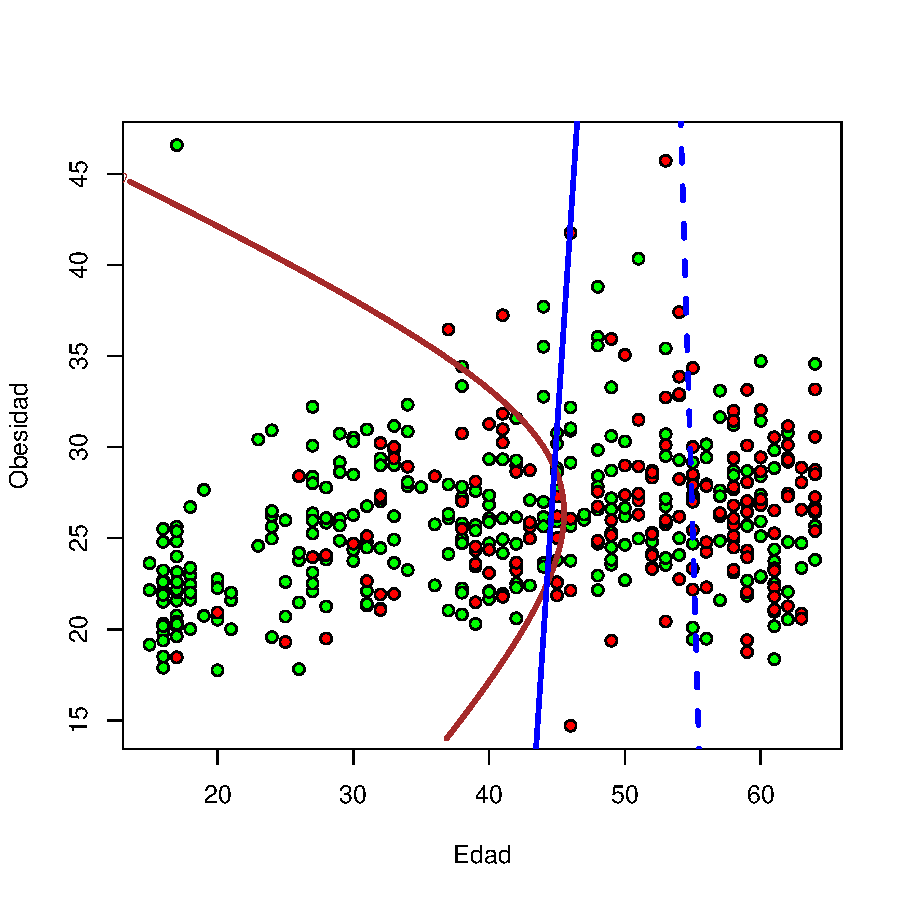
\includegraphics[height=8cm]{pdf/tema4/_edadobesidad-reglas-log}}

\section{Regla de Bayes}

Vamos a ver (en la tercera asignatura del grado) la regla de Bayes para clasificar.

Imaginemos que tenemos las probabilidades reales, entonces, $P(Y=1 | x) > P(Y=0 | x)$. 



En el caso en que 
\begin{enumerate}
\item $P_0$ tiene densidad $f_0$ y  $P_1$ tiene densidad $f_1$,
\item las \textbf{probabilidades a priori} de las poblaciones son
$$\mathbb{P}(P_0)=\pi_0,\quad \mathbb{P}(P_1)=\pi_1\quad (\pi_0+\pi_1=1).$$
\item Distribución condicionada de las variables explicativas: $P(X|Y=0) = 0$ tiene densidad $f_0$ y $P(X|Y=1)$ tiene densidad $f_1$.

\subitem Ahora, aplicamos la regla de bayes: \[P(Y=1 | X=x) = \frac{P(X=x|Y=1)P(Y=1)}{P(X=x)} = \frac{f_1(x)π_1}{π_0f_0(x) + π_1f_1(x)}\]
Por otro lado:
\[P(Y=0 | X=x) = \frac{P(X=x|Y=0)P(Y=0)}{P(X=x)} = \frac{f_0(x)π_0}{π_0f_0(x) + π_1f_1(x)}\]

\paragraph{Conclusión}
\[
\mathbb{P}(Y=1|x)>\mathbb{P}(Y=0|x) \Leftrightarrow \pi_1 f_1(x)>\pi_0 f_0(x).
\]
\end{enumerate}

\begin{prop}
La regla Bayes es óptima (su error de clasificación es el mínimo posible).
\end{prop}
\begin{proof}
No da tiempo a verlo, asique nos lo creemos.
\end{proof}
\subsection{Bayes para normalidad}

Supongamos que $f_0$ y $f_1$ son normales: para $x\in\mathbb{R}^p$,
\[
f_i(x) = |\Sigma_i|^{-1/2}(2\pi)^{-p/2}\exp\left\{-\frac{1}{2}(x-\mu_i)'\Sigma_i^{-1}(x-\mu_i)    \right\},\quad i=0,1.
\]


\textbf{Regla Bayes bajo normalidad}\\
$x$ en $P_0$ si $\displaystyle  d_{M_0}^2(x,\mu_0)<d^2_{M_1}(x,\mu_1)+2\log\left(\frac{\pi_0|\Sigma_1|^{1/2}}{\pi_1|\Sigma_0|^{1/2}}\right)$
donde $\displaystyle d_{M_i}^2(x,\mu_i)=(x-\mu_i)'\Sigma_i^{-1}(x-\mu_i)$ es el cuadrado de la distancia de Mahalanobis entre $x$ y $\mu_i$ ($i=0,1$).

La distancia de Mahalanobis aparece porque es lo que está en el argumento de la exponencial de la normal. Se deja como ejercicio el convencerse de esto.


\obs Vemos que esta regla se parece a la regla de Mahalanobis, solo que hay una constante que modifica la inecuación. Si esa constante fuera 0, tendríamos exactamente la regla de Mahalanobis.

¿Cuándo esa constante es 0? Cuando $Σ_0 = Σ_1$ (es decir, \textbf{Homocedasticidad}) y además, cuando $π_0 = π_1$, es decir, cuando las probabilidades a priori son iguales. 


\obs Ahora, nos venimos arriba y vamos a relacionarlo con la regla de Fisher:

\textbf{Regla bajo normalidad y homocedasticidad ($\Sigma_0=\Sigma_1$)}\\
$x$ se clasifica en $P_0$ si
$\displaystyle  w^\prime  x < w^\prime  \left(\frac{\mu_0+\mu_1}{2}\right)+  \log\left(\frac{\pi_0}{\pi_1}\right)$


Esto tiene algún parecido a la regla de Fisher.


\section{Regla óptima de clasificación bajo normalidad}

\begin{itemize}
  \item \textbf{Homocedasticidad} $Σ_1 = Σ_0 \to$ Regla de Fisher trasladada en función de $π_0$ y $π_1$.
  \item Cuando además de homocedasticidad, tenemos $π_0 = π_1$, la regla óptima es la regla de Fisher tal y como la hemos visto.
  \item $Σ_0 ≠ Σ_1 \to $ la distancia de Mahalanobis trasladada.
\end{itemize}


\begin{defn}[Error\IS Bayes]
El error bayes ($L^{*}$) es el menor error posible en una clasificación.
\end{defn}

\obs Dado que la regla de bayes es óptima, esta es una cota inferior para cualquier clasificador.